\documentclass[main.tex]{subfiles}

\begin{document}
Voltdb runs perfeclty in all modes and scale factors. But benchmarking app has a bug and cant gather final data for scale factor of 3 and 100 in write mode. oltpbenchmark cant connect properly to Postgres in scale facotor if 100 in all modes and, 5 and 10 for write mode, 3 and 5 and 10 for high read mode. It seemed that the main reason is that oltpbenchmark wants to create high connections  and Postgres rejects them. Also in some cases Postgres gets to its lock limits and in some cases high frequency of dead locks makes databse less effective.In all cases except high read mode in scale factor of 2, Voltdb acts better than Postgres. The main reason is Voltdb is first-based-memory dbms and intracts only a little with disk.\\
Postgres transaction latencies were close together and this shows stable and equal treatment with all terminals and requests.\\
\begin{minipage}{\textwidth}
    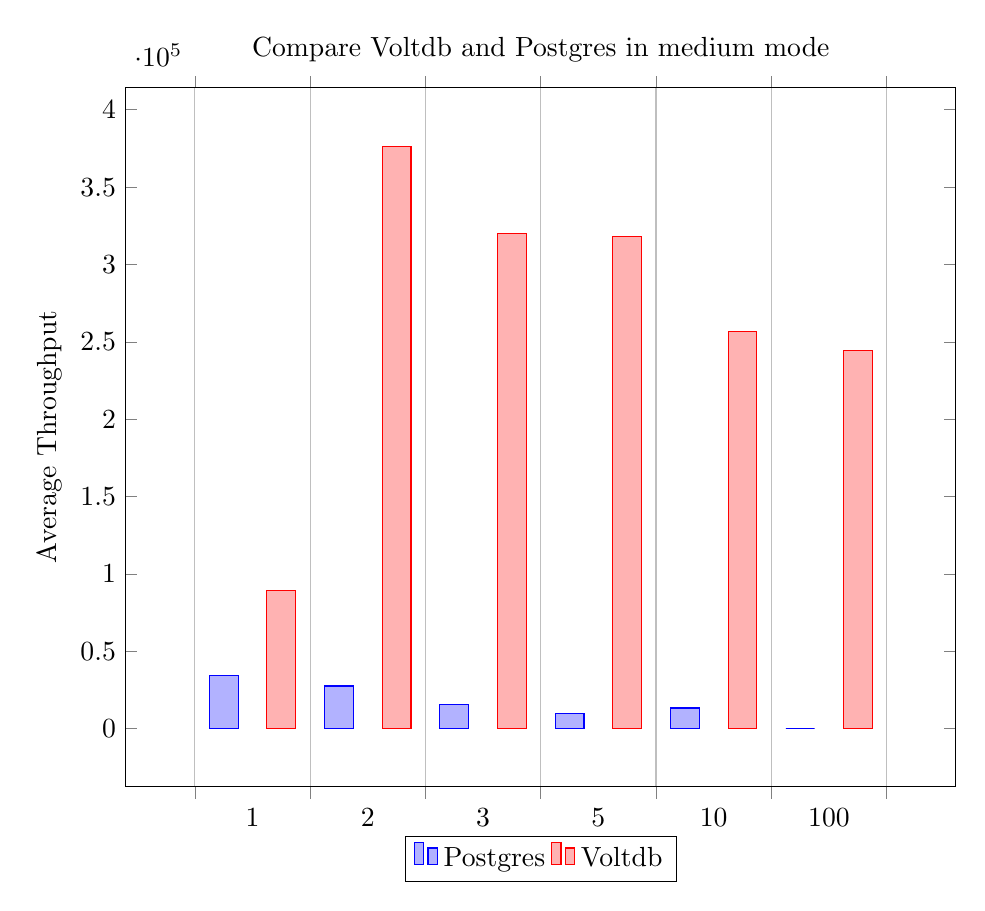
\begin{tikzpicture}
        \begin{axis}[
            ybar,
            title={Compare Voltdb and Postgres in medium mode},
            width=\textwidth,
            ybar interval=0.5,
            legend style={at={(0.5,-0.07)},
            anchor=north,legend columns=-1},
            ylabel={Average Throughput},
            symbolic x coords={1,2,3,5,10,100,dummy},
            ]
            \addplot coordinates { (1,34332.6) (2,27534.6) (3,15676.28) (5,9573.57) (10,13276.8) (100,0) (dummy,0) };
            \addplot coordinates { (1,89104) (2,376488) (3,319829) (5,317795) (10,256890) (100,244398) (dummy,0) };
            \legend{Postgres, Voltdb}
        \end{axis}
    \end{tikzpicture}
\end{minipage}
\begin{minipage}{\textwidth}
    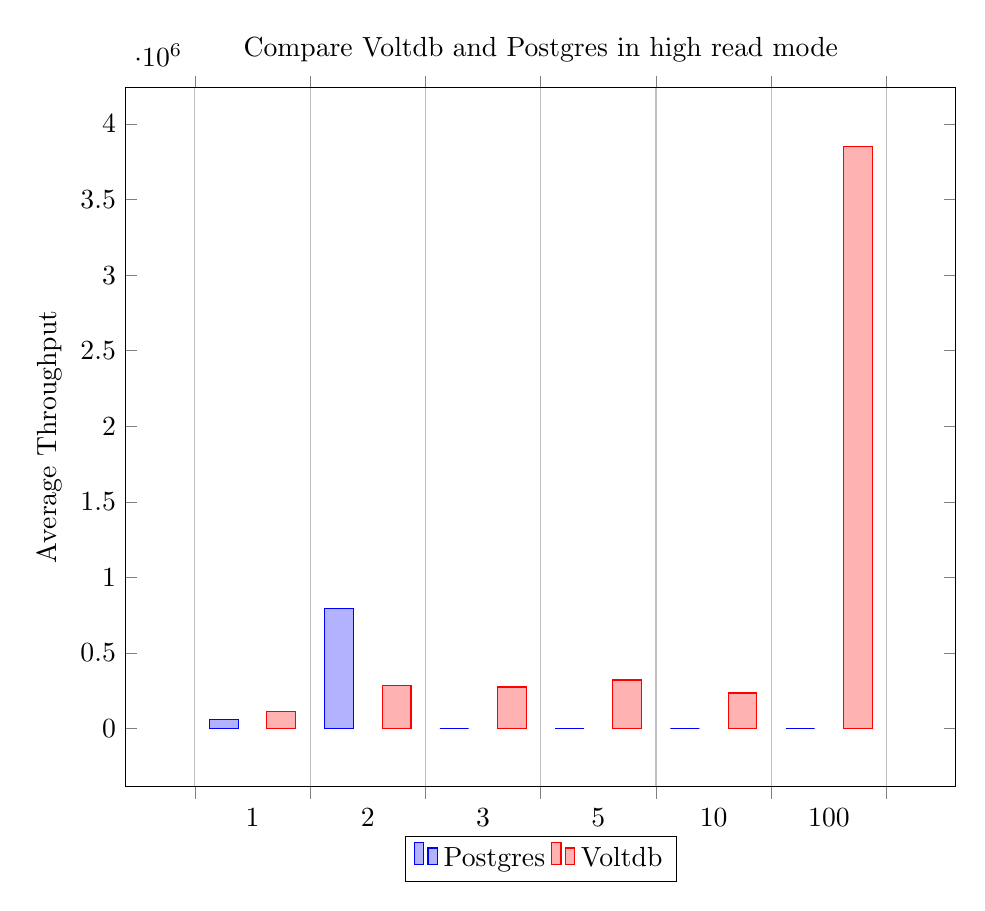
\begin{tikzpicture}
        \begin{axis}[
            ybar,
            title={Compare Voltdb and Postgres in high read mode},
            width=\textwidth,
            ybar interval=0.5,
            legend style={at={(0.5,-0.07)},
            anchor=north,legend columns=-1},
            ylabel={Average Throughput},
            symbolic x coords={1,2,3,5,10,100,dummy},
            ]
            \addplot coordinates { (1,59767) (2,796608) (3,0) (5,0) (10,0) (100,0) (dummy,0) };
            \addplot coordinates {  (1,111039) (2,286569) (3,275220) (5,321660) (10,235465) (100,3853688) (dummy,0) };
            \legend{Postgres, Voltdb}
        \end{axis}
    \end{tikzpicture}
\end{minipage}
\begin{minipage}{\textwidth}
    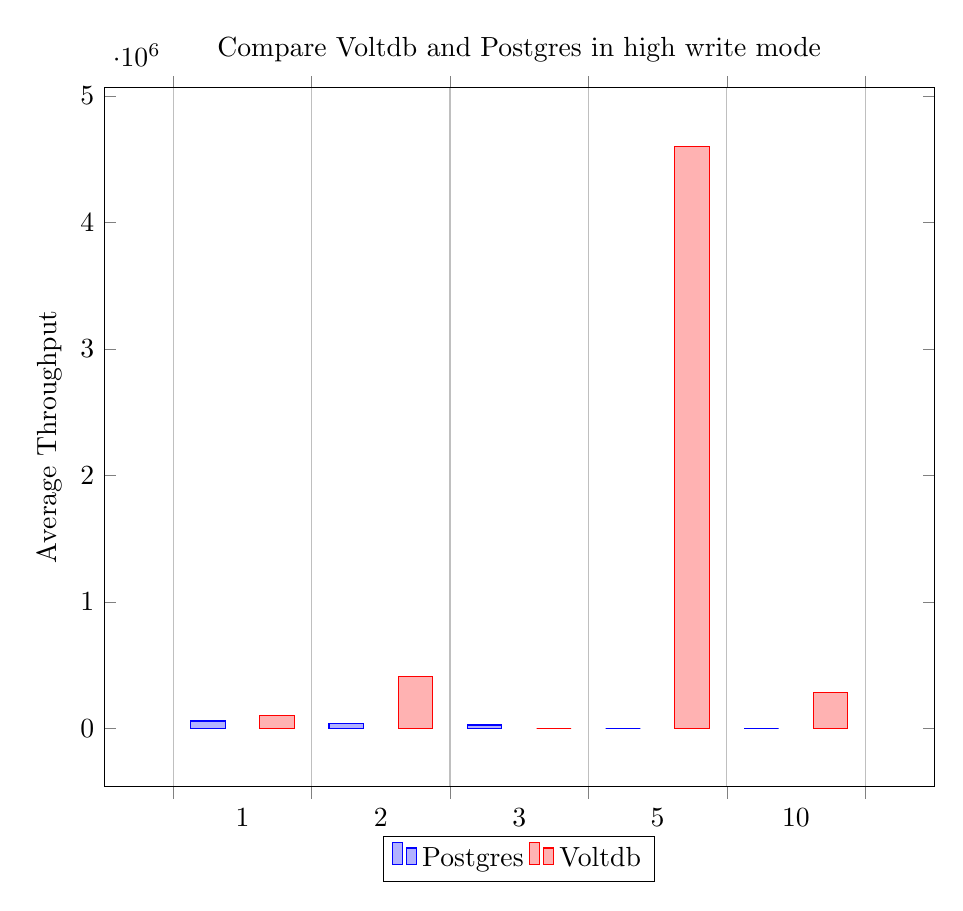
\begin{tikzpicture}
        \begin{axis}[
            ybar,
            title={Compare Voltdb and Postgres in high write mode},
            width=\textwidth,
            ybar interval=0.5,
            legend style={at={(0.5,-0.07)},
            anchor=north,legend columns=-1},
            ylabel={Average Throughput},
            symbolic x coords={1,2,3,5,10,dummy},
            ]
            \addplot coordinates { (1,59767) (2,43280.4) (3,27900) (5,0) (10,0) (dummy,0) };
            \addplot coordinates { (1,103493) (2,409570) (3,0) (5,4603719) (10,286881) (dummy,0) };
            \legend{Postgres, Voltdb}
        \end{axis}
    \end{tikzpicture}
\end{minipage}
\end{document}